\chapter{Glossar}

\newcommand{\term}[2]{
\vspace{1em}\noindent {\large \bfseries \color{seccol} \textsf{#1}}
\begin{addmargin}{1em}
#2
\end{addmargin}}


\term{AF}
{Audio Frequency, Töne im hörbaren Bereich. Auch NF (Niederfrequenz) genannt. 

Im Amateurfunk werden oftmals nur Frequenzen von 300 bis 3000 Hz übertragen, da dies für die Verständigung ausreichend ist und nicht übermässig viel Platz im Spektrum verschwendet. Die Bandbreite beträgt für ein solches Sprachsignal auf SSB $3000~\mathrm{Hz} - 300~\mathrm{Hz} = 2700~\mathrm{Hz}$.
}

\term{AGC}
{Der \textit{Automatic Gain Control} hält die AF auf einer bestimmten Stärke. Dies kann bei digitalen Übertragungsverfahren (RTTY, PSK) nützlich sein, da die Lautstärke konstant bleibt, bei CW ist er jedoch eher hinderlich, da während einer Sendepause das Rauschen gleich stark ist wie sonst das Signal.}

\term{AM}
{Siehe \plink{sec:am}{Amplitudenmodulation}}

\term{APRS}
{Automatic Position and Recording System – ein Zusammenspiel von GPS und Packet Radio.

144.800 MHz}

\term{Bake}
{Baken (wie zum Beispiel die \plink{sec:ncdxf}{NCDXF-Baken}) senden immer auf einer bestimmten Frequenz. So kann man sich ein Bild der aktuellen Ausbreitungsbedingungen machen.

Software: BeaconSee}

\term{Balun}
{Übergang von symmetrisch auf asymmetrisch (balanced – unbalanced). Beispiel: Übergang eines Dipols (symmetrisch) auf ein Koaxialkabel (asymmetrisch).}

\term{Beam}
{Anderer Name für eine \plink{sec:yagi}{Yagi-Antenne}.}

\term{Betriebsart}
{Die Betriebsart (also die Art, wie man Funkbetrieb macht) beinhaltet verschiedene Eigenschaften wie Verkehrsart (Simplex, Duplex, …), Modulation (AM, FM, …) und Übertragungsverfahren.}

\term{BFO}
{Der \textit{Beat Frequency Oscillator} generiert eine Trägerfrequenz, die bei Bedarf der ZF beigemischt wird. Beispielsweise wird dies bei CW oder SSB benötigt.

Im folgenden Beispiel wird ein CW-Signal dargestellt. 

%\begin{minipage}{55mm}
\begin{figure}[h!]
 \centering
 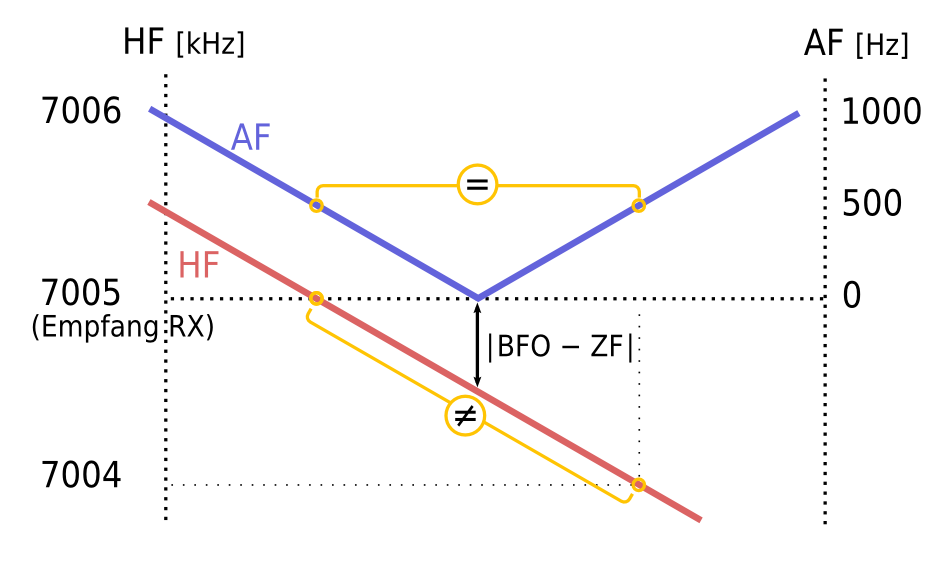
\includegraphics[width=5cm]{./png/Amfu-BFO.png}
 % Amfu-BFO.png: 929x581 pixel, 295dpi, 8.00x5.00 cm, bb=0 0 227 142
 \caption{Grosse Bandbreite: Ein CW-Signal auf 7005 kHz hat die selbe NF-Tonhöhe wie ein Signal auf 7004 kHz.}
 \label{fig:bfo}
\end{figure}
%\end{minipage}
%\begin{minipage}{55mm}
\begin{figure}[h!]
 \centering
 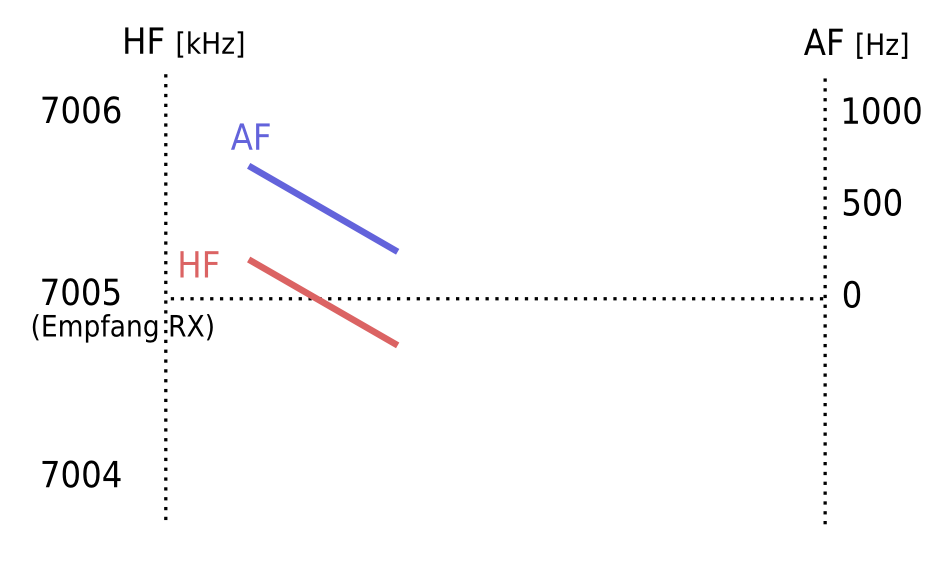
\includegraphics[width=5cm]{./png/Amfu-BFO-Filter.png}
 % Amfu-BFO-Filter.png: 929x581 pixel, 295dpi, 8.00x5.00 cm, bb=0 0 227 142
 \caption{Bei einer Bandbreite von 0.5 kHz verschwindet dieses Problem.}
 \label{fig:bfoFilter}
\end{figure}
%\end{minipage}



$f_d = |f_{\mathrm{BFO}}-f_{\mathrm{ZF}}|$ lässt sich beim Empfänger meist direkt einstellen. Ein Signal, das direkt auf der Empfangsfrequenz liegt, wird dann mit dieser NF hörbar gemacht. Andernfalls wird der Abstand zur Eingangsfrequenz addiert oder subtrahiert: $|f_d + (f_\mathrm{Signal}-f_\mathrm{RX})|$.

Das ist auch der Grund, warum beim Scannen eines CW-Bandes die einen Signale höher, die andern tiefer werden. Beim Empfang eines breiten Spektrums haben zwei Signale, die $2\times \mathrm{f_d}$ auseinander liegen, die selbe AF-Tonhöhe! Darum verschwinden einige Signale beim verringern der Bandbreite, da sie zwar die eingestellte fd-Tonhöhe haben, aber um die zweifache fd-Frequenz weiter unten liegen. Sobald die Bandbreite unter $2\times \mathrm{f_d}$  liegt, hat man diese Probleme nicht mehr.}

\term{Bodenwelle}
{Der Teil einer elektromagnetischen Welle, der sich über den Boden ausbreitet. Siehe \plink{sec:bodenwelle}{Bodenwelle}}

\term{CB}
{Abkürzung für \textit{Citizen Band}. Auf diesem HF-Band um 27 MHz kann, ähnlich wie bei PMR, ohne Lizenz gefunkt werden.}

\term{CTCSS}
{CTCSS \textit{(Continious Tone Code Squelch System)} moduliert einen NF-Ton unter 300 Hz (\link{Subaudio}-Ton) mit dem FM-Träger. CTCSS wird gerne von Relais benutzt, da damit ungewollte Aktivierungen, z. B. von Radars oder durch Nebenaussendungen anderer Stationen, verhindert werden können: Es öffnet nur, wenn der richtige Ton moduliert wird.

Insgesamt werden 50 verschiedene Töne von 67 bis 254.1 Hz verwendet.}

\term{Dämpfung}
{Die Dämpfung bzw. Verstärkung (Kabel, Antenne, …) wird in Dezibel (dB) angegeben. Für Koaxialkabel gilt der Wert jeweils für 100 m.}

\term{DCS}
{DCS (Digital Code Squelch) funktioniert ähnlich wie \link{CTCSS}: Der Empfänger wird geöffnet, sobald das richtige Signal am HF-Eingang liegt. DCS arbeitet jedoch mit einem FSK-Stream im Subaudio-Bereich, mit dem Daten (bzw. bestimmte Codes) übertragen werden. Das System ist so weniger störanfällig.}

\term{Dezibel}
{Es können sowohl relative Angaben zur Verstärkung bzw. Dämpfung als auch absolute bei Pegeln verwendet werden. dB-Werte sind addierbar, was die Errechnung des Gesamtgewinnes aus Antenne, Kabel- und Steckerverlust vereinfacht.
Bei der Angabe von Leistungspegeln gilt:

\[ a_\mathrm{dBm} = 10 \cdot \log \frac{P}{P_\mathrm{ref}} \]

Für Spannungspegel:

\[ a_\mathrm{dBµV} = 20 \cdot \log \frac{U}{U_\mathrm{ref}} \]

Eine Verstärkung der Leistung um 3 dB bedeutet eine Leistungsverdoppelung. Zwei Antennen mit je 3 dB Gewinn erbringen zusammen einen Gewinn von $3 + 3 = 6~\mathrm{dB}$ (also das Vierfache).

Nähere Beschreibung in der \link{Formelsammlung}.}

\term{DTMF}
{DTMF (Dual Tone Multiple Frequency), auch MFV – Mehrfrequenzwahlverfahren – genannt, wird zum aktivieren von Relais und für die Auswahl von \link{Echolink}-Repeatern verwendet. Die meisten EL-Relais verlangen zuerst einen \textbf{*}, um EL zu aktivieren, bevor die Node-Nummer eingegeben wird. Die Raute (\textbf{\#}) beendet die Verbindung wieder.}

\term{Dipol}
{Ein Antennendraht der Länge $\lambda/2$. Siehe \plink{sec:dipol}{Dipol}.}

\term{Doppelsuper}
{Empfänger mit zwei Zwischenfrequenzen: Eine hohe erste ZF, die die Spiegelfrequenz unterdrückt, und eine zweite tiefe ZF, die eine gute Trennschärfe erlaubt. }

\term{Echolink}
{\href{http://www.echolink.org}{www.echolink.org} – Webauftritt von Echolink

Mit Echolink lassen sich Funkverbindungen zwischen zwei Benutzern «übers Internet» erstellen. Auf das Echolink-System kann man entweder vom PC aus\footnote{Software ist momentan nur für Windows erhältlich.} (VoIP-ähnlich) oder über ein Relais, das Echolink (EL) unterstützt, zugreifen. 

Sowohl Benutzer am PC als auch Relais bekommen eine ID zugewiesen. Zwischen zwei IDs kann eine Verbindung hergestellt werden; PC-Benutzer können so direkt angesprochen werden, auch über Funk.

Ein häufiger Verwendungszweck von Echolink ist die Erstellung einer Verbindung zwischen zwei Relais, die beliebig weit voneinander entfernt sein können, da Verbindungen zwischen zwei IDs digital übers Internet erfolgt.

\vspace{1em}
\begin{tabular}{ll}
\bfseries Input & \\ \toprule \arrayrulecolor{rowsep}
Nummer & Verbindet mit dem gewählten Node \\ \midrule
\# & Unterbricht die aktive Verbindung \\ \midrule
* & Stationsinfo, wenn nicht verbunden \\ \midrule
0 & Verbindet mit zufälliger Station jeden Typs \\ \midrule
1 & Verbindet mit zufälligem -L (Link) oder -R (Repeater) \\ \midrule
2 & Verbindet mit zufälligem Konferenzserver \\ \midrule
3 & Verbindet mit zufälligem Benutzer \\ \midrule
06 Nr. & Statusinfo zur gewählten Nummer \\ \midrule
8 & Gibt die Rufzeichen der verbundenen Stationen aus  \\ \midrule
9 & Wiederwahl zu zuletzt gewählter Station \\ \midrule
\end{tabular}
}


\term{FM}
{\link{Frequenzmodulation, S. 37}}

\term{FRS}
{Family Radio Service; Amerikanisches PMR.}

\term{Fuchsjagd}
{Amateurfunkpeilen. Ähnlich wie bei einem OL müssen Sender, die auf einer bestimmten Frequenz senden, gefunden werden. Durch mehrere Peilungen können sie geortet und auf einer Karte eingetragen werden. \link{Formelsammlung}}

\term{Ground wave}
{\link{Bodenwelle, Seite 33}}

\term{Hochpass}
{Filter aus Kondensatoren und Spulen, das hohe Frequenzen passieren lässt. Wird auch eingesetzt, um den 50-Hz-Brumm der Steckdose zu entfernen.}

\term{ITU}
{Die \textit{International Telecommunication Union}, auf Deutsch Internationale Fernmeldeunion. }

\term{Koax}
{Koaxialkabel (siehe \plink{koax}{Koaxialkabel}) wird für die Übertragung der Signale zwischen Antenne und Empfänger verwendet. Die gebräuchlichsten Arten sind RG58 (5.8 mm Durchmesser) und RG213 (10.3 mm Durchmesser).

Für Amateurfunk verwendet man eigentlich nur 50-$\Omega$-Kabel. 75-Ohmiges wird im Fernsehbereich eingesetzt. Bei höheren Frequenzen wird aufgrund des \link{Skin-Effektes} dickeres Kabel (RG213) eingesetzt.
}

\term{Koax-Steckverbindungen}
{Häufige Steckverbindungen: BNC, N und UHF/PL. BNC findet man oft an RG58-Kabel, N wird eher für das dicke RG213 verwendet (VHF/UHF). PL-Stecker sind nur für Frequenzen bis ungefähr 200 MHz geeignet.}

\term{Kyrillisch}
{Im kyrillischen Alphabet haben «unsere» Buchstaben eine andere Bedeutung. In folgender Tabelle jeweils links der kyrillische Buchstabe und rechts das lateinische Morsezeichen (die Morsezeichen sind in den Bakom-Vorschriften angegeben).

\vspace{1em}
\begin{tabular}{l>{\bfseries}l l>{\bfseries}l l>{\bfseries}l}
\ru{А а} & a & \ru{К к} & k & \ru{Х х} & h \\ \midrule
\ru{Б б} & b & \ru{Л л} & l & \ru{Ц ц} & c \\ \midrule
\ru{В в} & w & \ru{М м} & m & \ru{Ч ч} & ö \\ \midrule
\ru{Г г} & g & \ru{Н н} & n & \ru{Ш ш} & ch \\ \midrule
\ru{Д д} & d & \ru{О о} & o & \ru{Щ щ} & q \\ \midrule
\ru{Е е} & e & \ru{П п} & p & \ru{Ъ ъ} & x \\ \midrule
\ru{Ё ё} & e & \ru{Р р} & r & \ru{Ы ы} & y \\ \midrule
\ru{Ж ж} & v & \ru{С с} & s & \ru{Ь ь} & x \\ \midrule
\ru{З з} & z & \ru{Т т} & t & \ru{Э э} & é \\ \midrule
\ru{И и} & i & \ru{У у} & u & \ru{Ю ю} & ü \\ \midrule
\ru{Й й} & j & \ru{Ф ф} & f & \ru{Я я} & ä \\ \midrule
\end{tabular}


}

\term{Locator}
{\link{Maidenhead-Locator}}

\term{LUF}
{Die Lowest Usable Frequency ist die tiefste Frequenz, die zwischen zwei Punkten genutzt werden kann. Sie ist von der Ionisierung der D- und E-Schicht und daher auch von der Tageszeit abhängig.}

\term{Maidenhead-Locator}
{Im Amateurfunk wird für die Positionsangabe ein eigenes System verwendet. Die Welt wird in $18\times 18$ Grösstfelder (\textit{Fields}, A…R), $10\times 10$ Grossfelder (\textit{Squares}, 0…9) und $24\times 24$ Kleinfelder (\textit{Subsquares}, a…x) unterteilt, feinere Unterteilungen sind möglich. Das erste Zeichen gibt jeweils die Länge an, das zweite die Breite. Beispiel: JN47qh

\begin{figure}[h!]
 \centering
 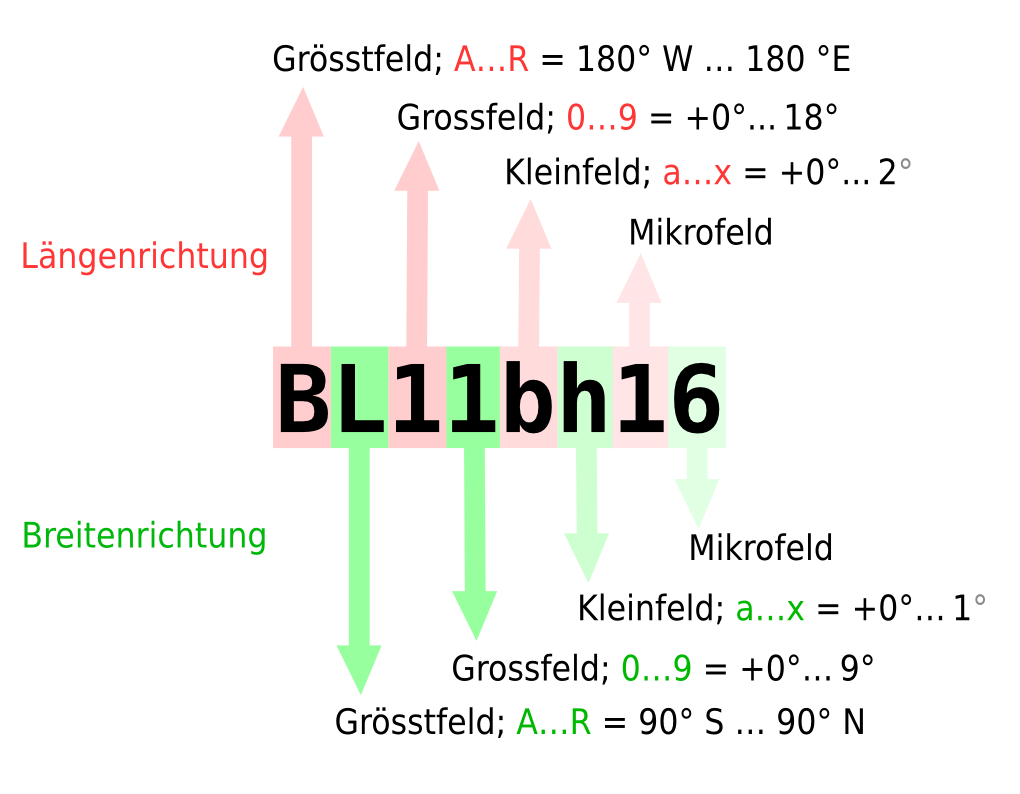
\includegraphics[width=6cm]{./png/Maidenhead_QTH-Locator_erklaert.png}
 \caption{Aufbau des Maidenhead-Locators}
 \label{fig:maidenhead}
\end{figure}

}

\term{Modulationsindex}
{Verhältnis von Hubfrequenz zur maximalen Niederfrequenz}

\term{MUF}
{Die Maximal Usable Frequency liegt wenig unter der höchsten Frequenz, die an der F-Schicht der Ionosphäre noch reflektiert wird. Tagsüber ist sie höher als bei Nacht. Ausserdem ist sie abhängig vom Abstrahlwinkel: Bei sehr guten Bedingungen und einem Abstrahlwinkel um 0° können Frequenzen von bis zu 70 MHz reflektiert werden.

Sonden, die die MUF messen, senden ein Signal zur Erde, das dann reflektiert wird. Da es senkrecht auf die Ionosphäre auftrifft, ist die so erhaltene MUF niedriger. Die 0°-MUF kann daraus hochgerechnet werden – für das $F_2$-Band beträgt sie das 2.5- bis 3.5-fache.}

\term{Netzeinströmung}
{Beim Senden kann es geschehen, dass ein Teil der Energie ins Stromnetz einströmt und so zu Störungen anderer Geräte führt. Dies kann verhindert werden, indem man das Stromkabel um einen Ferritring wickelt. Grundsätzlich gilt: Je mehr Windungen, desto besser, aber ein Viertel des Ferrites sollte frei bleiben.}

\term{NF}
{\link{AF}}

\term{Notchfilter}
{Ein Notchfilter (Saugkreis) filtert eine HF-Frequenz heraus.

\begin{figure}[h!]
 \centering
 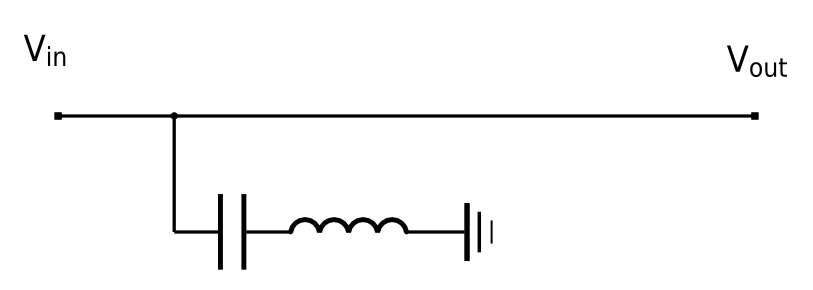
\includegraphics[width=4cm]{./png/Amfu-Schema-Notchfilter.png}
 % Amfu-Schema-Notchfilter.png: 813x290 pixel, 295dpi, 7.00x2.50 cm, bb=0 0 198 71
 \caption{Einfacher Notchfilter: Serieschwingkreis}
 \label{fig:notchfilter}
\end{figure}

Nach dem selben Prinzip funktionieren einstellbare, schmalbandigere Notchfilter später im Empfänger. Dies ist vor allem nützlich, wenn eine andere Station stört.

Ein einfacher Notchfilter lässt sich mit einer Spule und einem Kondensator realisieren, die in Serie geschaltet und zwischen Antenne und Erde gehängt werden. Für den NF-Bereich wird anstelle einer Spule ein Widerstand eingebaut, da für tiefe Frequenzen eine grosse Induktivität notwendig wäre.

\begin{figure}[h!]
 \centering
 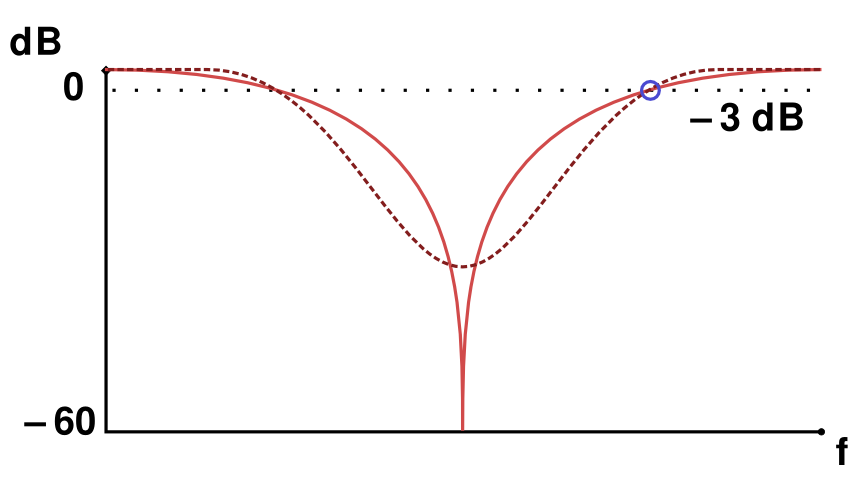
\includegraphics[width=5cm]{./png/Amfu-Notchfilter.png}
 % Amfu-Notchfilter.png: 864x480 pixel, 288dpi, 7.62x4.23 cm, bb=0 0 216 120
 \caption{Dämpfungskurven: Notchfilter und 
(gestrichelt) Bandsperre}
 \label{fig:notchfilterFreq}
\end{figure}
}

\term{Öffnungswinkel}
{Der Öffnungswinkel einer Antenne ist der Winkelabstand zwischen zwei Punkten, bei denen der Gewinn um 3 dB abgefallen ist. Ein Yagi hat einen kleineren Öffnungswinkel als ein Dipol.}

\term{Ortung}
{Positionsbestimmung eines Signals durch zwei oder mehr \link{Peilungen}.}

\term{Peilung}
{Richtungsbestimmung eines Signals. Für \link{Fuchsjagden} wird dazu meist eine Loop verwendet, für HF werden stationäre Peiler mit mehreren GPs, in einem Kreis angeordnet, eingesetzt.}

\term{Pile-up}
{Ein Effekt, der bei speziellen Stationen oder bei Contests auftritt, wenn mehrere Stationen mit einer bestimmten eine Verbindung herstellen möchten.}

\term{PMR}
{PMR \textit{(Private Mobile Radio)} bezeichnet den «Funk für Jedermann»: Hier darf ohne Amateurfunklizenz gefunkt werden. Auf den PMR-Geräten sind 8 verschiedene Kanäle verfügbar, auf denen mit FM und halbem Hub (für eine geringere Leistungsaufnahme und höhere Kanaldichte) gefunkt wird.

Auf den PMR-Frequenzen (446–446.1 MHz) dürfen alle geprüften PMR-Handfunkgeräte mit bis zu 500 mW senden. Amateurfunkgeräte sind normalerweise nicht für diese Kanäle geprüft und erlauben es darum im unmodifizierten Zustand auch nicht, dort zu funken.}

\term{Polarisation}
{Bei Antennen unterscheidet man zwischen horizontaler und vertikaler Polarisation des elektrischen Feldes. Für einen optimalen Empfang sollte die Polarisation zweier Stationen übereinstimmen. Dipole sind grundsätzlich horizontal, GPs vertikal polarisiert.

\begin{figure}[h!]
 \centering
 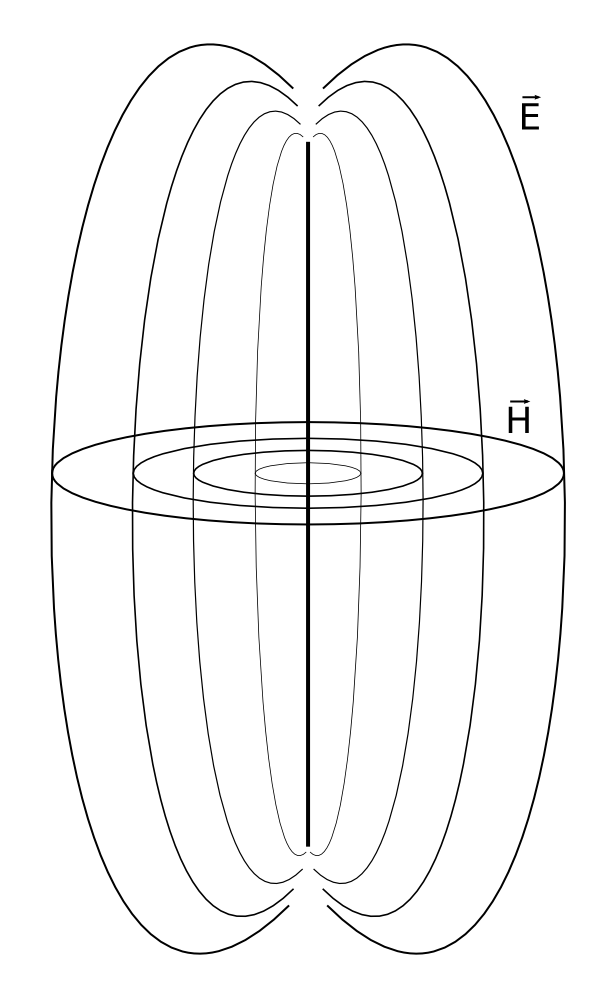
\includegraphics[height=5cm]{./png/Amfu-Antenne-Polarisation.png}
 % Amfu-Antenne-Polarisation.png: 612x1008 pixel, 360dpi, 4.32x7.11 cm, bb=0 0 122 202
 \caption{GP, vertikal polarisiert}
 \label{fig:polarisation}
\end{figure}

}

\term{QRN}
{QRN entsteht durch atmosphärische Störungen wie Gewitter (Blitze sind auf dem gesamten Spektrum hörbar!) und kann den Funkverkehr erheblich beeinträchtigen. Andererseits kann genau dies zum Beispiel auch zum Zählen von Blitzen verwendet werden.

Nicht zu verwechseln mit QRM \textit{(man-made noise)}, Störungen, die etwa durch ein schlechtes Netzteil (Brummton) oder diverse elektrische Geräte hervorgerufen werden können.}

\term{Raumwelle}
{\link{Raumwelle, Seite 33}}

\term{Rauschsperre}
{Squelch}

\term{RG-58}
{Koaxialkabeltyp, der gerne für HF eingesetzt wird. Der Wellenwiderstand beträgt $58~\Omega$ und der Verkürzungsfaktor 0.66.}

\term{RIT}
{Das \textit{Receiver Incremental Tuning} (auch \textit{Clarifier} genannt) wird eingesetzt, wenn eine empfangene Station keinen stabilen Sender hat und sich dessen Frequenz langsam verändert (die von ihm empfangene Frequenz jedoch nicht!). Beim RIT wird nur die Eingangsfrequenz verstellt; so ist es möglich, auf der selben Frequenz zu senden, aber etwas daneben zu hören.

RIT wird oft auch von raren DX-peditions gebraucht, welche nach dem CQ-Ruf z. B. «up 2» geben (das heisst, sie wollen, dass man sie 2 kHz weiter oben ruft, um das Pile-up besser in
den Griff zu bekommen).}

\term{Schwund}
{Wird von einem Signal mehr als eine Reflexion empfangen, führt das zu starken Schwankungen der Signalstärke.}

\term{Sferics}
{Kommt von \textit{atmospherics}. \link{Blitze, Seite 34}}

\term{Signal-Rausch-Abstand}
{SNR. \link{Formelsammlung}}

\term{Skin-Effekt}
{Ein Leiter (zum Beispiel ein Kupferkabel) zeigt bei Gleichstrom eine gleichmässige Stromverteilung. Bei Wechselstrom werden die Elektronen aufgrund des Magnetfeldes, das durch die Mitte des Leiters geht, nach aussen verdrängt. So steigt der Widerstand etwa bei 10 MHz bereits um das 10-fache an (Kupferdraht, $1~\mathrm{mm}^2$). Abhilfe schafft Litzendraht (mehrere feine Drähte haben leicht bessere Eigenschhaften) oder, noch besser, ein dickerer Leiter.}

\term{Sky wave}
{\link{Raumwelle, Seite 33}}

\term{Spektrogramm}
{Ein Spektrogramm, beziehungsweise eine Spektrumanalyse, zeigt zu einer bestimmten Zeitspanne die Verteilung der Signalstärken im analysierten Frequenzband auf. Beispiel: \link{Grafik 5, Seite 36.}

Berechnet wird das Spektrogramm mittels FFT \textit{(Fast Fourier Transformation)}. Frequenz und Zeit können dabei aufgrund der Unschärferelation nicht gleichzeitig exakt bestimmt werden.}

\term{Sperrkreis}
{Der Sperrkreis (Parallelschwingkreis) hat eine andere Dämpfungskurve als der \link{Notchfilter}. Sie werden oft zusammen verwendet.

\begin{figure}[h!]
 \centering
 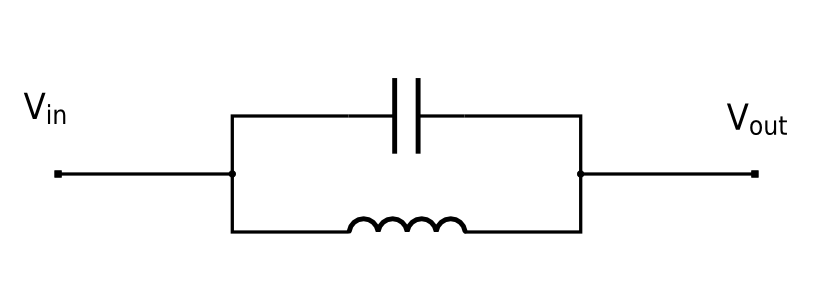
\includegraphics[width=4cm]{./png/Amfu-Schema_Sperrkreis.png}
 % Amfu-Schema_Sperrkreis.png: 813x290 pixel, 295dpi, 7.00x2.50 cm, bb=0 0 198 71
 \caption{Schaltschema einer Bandsperre}
 \label{fig:sperrkreis}
\end{figure}

}

\term{Squelch}
{Der Squelch (Rauschsperre) sperrt den NF-Verstärker, solange das Signal im ZF-Verstärker einen bestimmten, einstellbaren Wert nicht überschreitet. So ist der Empfang etwas angenehmer (speziell für FM), da bei Sendepausen kein Rauschen hörbar ist, und bei Handfunkgeräten wird die Betriebsdauer verlängert. Bei schwachen Signalen, die unter dem Rauschpegel liegen, funktioniert der Squelch nicht (bzw. sperrt immer).

Bei oft benutzten Relais kann man zudem mit einem \link{Subaudio-Ton} arbeiten, der am Gerät eingestellt wird. Der Empfänger verstärkt dann nur empfangene Aussendungen, die diesen CTCSS-Ton enthalten \textit{(Tone Squelch)}. Die Frequenzen dieser «privaten» CTCSS-Töne werden untereinander ausgetauscht.

Die Rauschsperre findet vor allem bei FM Einsatz, da das Rauschen lauter als das Sprachsignal ist. Bei AM wird sie zum Sperren von Störungen verwendet.}

\term{SSB}
{\link{SSB, S. 37}}

\term{Subaudio-Ton}
{Ein Ton, dessen Frequenz unterhalb der hörbaren Frequenzen (\link{AF}) liegt. Er kann etwa zur Datenübertragung mitgesendet werden.}

\term{SWR}
{Stehwellenverhältnis, auch VSWR für Vorwärts-SWR. Je höher das SWR, desto mehr Leistung wird von der Antenne zurückgeworfen und geht als Wärme verloren. Es wird berechnet, indem man die maximale durch die minimale Leistung teilt:

\[\mathrm{SWR} = \frac{U_\mathrm{hin} + U_\mathrm{rück}}{U_\mathrm{hin}-U_\mathrm{rück}}\]
}

\term{Tiefpass}
{Wie ein Hochpass, lässt aber tiefe Frequenzen passieren. \link{Formelsammlung}}

\term{Tone Call}
{Auch \textit{T-Call} genannt. Ein Ton mit einer Frequenz von 1750 Hz, der zum Aktivieren von Relais verwendet werden kann.}

\term{Tote Zone}
{Die tote Zone ist ein Bereich zwischen dem Ende der Bodenwelle und dem ersten Auftreffen der reflektierten Raumwelle, in dem ein Signal nicht empfangen werden kann.}

\term{Tuner}
{Ein Gerät, das die Ausgangsimpedanz des Senders an die Impedanz der Antenne anpasst, um so eine optimale Leistungsübertragung zu ermöglichen.}

\term{Übertragungsverfahren}
{Bezeichnet die Art, wie etwas übertragen wird. Als Beispiel: CW, SSTV, PSK31. \link{Übertragungsverfahren, Seite 40} und \link{Betriebsart}}

\term{UTC}
{\link{UTC, Seite 10}}

\term{Verkürzungsfaktor}
{Elektromagnetische Signale bewegen sich nur im luftleeren Raum mit Lichtgeschwindigkeit fort. In anderen Materialien (speziell Antennendraht und -Kabel) ist die Fortbewegungsgeschwindigkeit niedriger, daher muss zum Beispiel die Drahtlänge eines 80-m-Dipols um einen Meter verkürzt werden.
}

\term{Verstärkung}
{\link{Dämpfung}}

\term{Wasserfalldiagramm}
{Der Wasserfall ist eine erweiterte Form des Spektrogramms. Die Signalstärke wird farblich hervorgehoben, dafür wird die dadurch frei gewordene Achse als Zeitachse verwendet. So ist es möglich, Frequenz, Zeit und Signalstärke gleichzeitig in einer zweidimensionalen Grafik darzustellen.  Beispiel: \link{Grafik 12, Seite 40}. \link{Spektrogramm}.

Heute findet der Wasserfall speziell bei digitalen Übertragungsverfahren wie PSK31 Verwendung, da so einzelne PSK-Signale schnell erkannt werden können.}

\term{Yagi}
{Eine \link{Yagi (S. 43)} ist eine Richtantenne.}

\term{Zwischenfrequenz}
{Die Zwischenfrequenz (ZF) ist der Abstand von der Oszillator- zur Eingangsfrequenz bzw. von der Oszillator- zur Spiegel­fre­quenz.}